% ============================================================
%  يُترجَم بـ XeLaTeX  (في Overleaf: Menu → Compiler → XeLaTeX)
%  الخط: Amiri (متوفر في Overleaf، أو حمّله من github.com/aliftype/amiri)
% ============================================================
\documentclass[12pt,a4paper]{article}
\usepackage[a4paper,margin=1.7cm,top=2.3cm,bottom=2.9cm,headheight=15pt,footskip=1.5cm]{geometry}
\usepackage{amsmath,amssymb}
\usepackage{icomma}
\usepackage[english,bidi=default,layout=lists]{babel}
\babelprovide[import,main]{arabic}
\babelfont{rm}[Scale=1.08]{Amiri}
\babelfont{sf}[Scale=1.08]{Amiri}
\usepackage[most]{tcolorbox}
\usepackage{tikz}
\usetikzlibrary{arrows.meta,calc,shadings}
\usepackage{array}
\usepackage{colortbl}
\usepackage{fancyhdr}
\usepackage{titlesec}
\usepackage{enumitem}
\usepackage{collcell}
\usepackage{needspace}
\usepackage{etoolbox}
\newcolumntype{C}{>{\collectcell\ar}c<{\endcollectcell}}
\pretocmd{\section}{\Needspace{15\baselineskip}}{}{}
\pretocmd{\subsection}{\Needspace{11\baselineskip}}{}{}

\definecolor{cDef}{HTML}{1F4E9C}
\definecolor{cThm}{HTML}{B3261E}
\definecolor{cRem}{HTML}{2E7D32}
\definecolor{cEx}{HTML}{C76B00}
\definecolor{cMeth}{HTML}{6A1B9A}
\definecolor{cSol}{HTML}{00695C}
\definecolor{cSec}{HTML}{1F3A68}

\titleformat{\section}{\Large\bfseries\color{cSec}}{\thesection.}{0.6em}{}[{\color{cSec!60}\titlerule[1pt]}]
\titleformat{\subsection}{\large\bfseries\color{cThm!85!black}}{\thesubsection.}{0.5em}{}
\titlespacing*{\section}{0pt}{14pt}{8pt}
\titlespacing*{\subsection}{0pt}{10pt}{5pt}
\setlength{\parindent}{0pt}
\setlength{\parskip}{4pt}
\setlist{itemsep=2pt,topsep=3pt}

\newtcolorbox{arbox}[3][]{enhanced,
  colback=#2!5,colframe=#2!80!black,arc=2mm,boxrule=0.8pt,
  left=6pt,right=6pt,top=8pt,bottom=5pt,
  fonttitle=\bfseries,coltitle=white,
  title={\foreignlanguage{arabic}{#3}},
  attach boxed title to top right={xshift=-5mm,yshift=-3mm},
  boxed title style={colback=#2!80!black,arc=1.5mm,boxrule=0pt},
  before upper={\selectlanguage{arabic}},
  before skip=8pt,after skip=8pt,breakable,#1}
\newenvironment{BOX}[2]{\begin{otherlanguage}{english}\begin{arbox}{#1}{#2}}{\end{arbox}\end{otherlanguage}}
\newenvironment{tarif}[1][تعريف]{\begin{BOX}{cDef}{#1}}{\end{BOX}}
\newenvironment{khassia}[1][خاصية]{\begin{BOX}{cThm}{#1}}{\end{BOX}}
\newenvironment{molahada}[1][ملاحظة]{\begin{BOX}{cRem}{#1}}{\end{BOX}}
\newenvironment{mithal}[1][مثال]{\begin{BOX}{cEx}{#1}}{\end{BOX}}
\newenvironment{tariqa}[1][طريقة]{\begin{BOX}{cMeth}{#1}}{\end{BOX}}

\newcounter{exo}
\newenvironment{tamrin}[1]{\stepcounter{exo}\begin{BOX}{cSec}{التمرين \theexo: #1}}{\end{BOX}}
\newenvironment{hal}{\Needspace{12\baselineskip}\begin{otherlanguage}{english}\begin{arbox}[breakable]{cSol}{حل التمرين \theexo}}{\end{arbox}\end{otherlanguage}}

\newenvironment{LTR}{\begin{otherlanguage}{english}}{\end{otherlanguage}}
\newcommand{\ar}[1]{\foreignlanguage{arabic}{#1}}

\renewcommand{\dots}{\mathinner{\ldotp\ldotp\ldotp}}
\renewcommand{\ldots}{\mathinner{\ldotp\ldotp\ldotp}}
\renewcommand{\cdots}{\mathinner{\cdotp\cdotp\cdotp}}
\newcommand{\N}{\mathbb{N}}
\newcommand{\Z}{\mathbb{Z}}
\newcommand{\D}{\mathbb{D}}
\newcommand{\Q}{\mathbb{Q}}
\newcommand{\R}{\mathbb{R}}
\newcommand{\pgcd}{\operatorname{PGCD}}
\newcommand{\ppcm}{\operatorname{PPCM}}

% \NLseg{a}{b}{[}{]} ; \NLright{a}{[} ; \NLleft{b}{]}  (interval on a number line)
\newcommand{\NLseg}[4]{\begin{LTR}\begin{tikzpicture}[baseline=-0.6ex]
 \draw[-{Stealth[length=2mm]},gray!70](0,0)--(3.4,0);
 \draw[line width=2pt,cThm!80!black](0.7,0)--(2.7,0);
 \node[cThm!80!black,font=\LARGE] at (0.7,0){$#3$};
 \node[cThm!80!black,font=\LARGE] at (2.7,0){$#4$};
 \node[below=3pt,font=\footnotesize] at (0.7,0){$#1$};
 \node[below=3pt,font=\footnotesize] at (2.7,0){$#2$};
\end{tikzpicture}\end{LTR}}
\newcommand{\NLright}[2]{\begin{LTR}\begin{tikzpicture}[baseline=-0.6ex]
 \draw[-{Stealth[length=2mm]},gray!70](0,0)--(3.4,0);
 \draw[line width=2pt,cThm!80!black](1.3,0)--(3.3,0);
 \node[cThm!80!black,font=\LARGE] at (1.3,0){$#2$};
 \node[below=3pt,font=\footnotesize] at (1.3,0){$#1$};
\end{tikzpicture}\end{LTR}}
\newcommand{\NLleft}[2]{\begin{LTR}\begin{tikzpicture}[baseline=-0.6ex]
 \draw[-{Stealth[length=2mm]},gray!70](0,0)--(3.4,0);
 \draw[line width=2pt,cThm!80!black](0.05,0)--(2.1,0);
 \node[cThm!80!black,font=\LARGE] at (2.1,0){$#2$};
 \node[below=3pt,font=\footnotesize] at (2.1,0){$#1$};
\end{tikzpicture}\end{LTR}}

% ---------- social-media icons (pure TikZ) ----------
\definecolor{cFB}{HTML}{1877F2}
\definecolor{cTG}{HTML}{229ED9}
\definecolor{cIG1}{HTML}{FEDA75}
\definecolor{cIG2}{HTML}{D62976}
\definecolor{cIG3}{HTML}{4F5BD5}
\newcommand{\fbicon}{\begin{LTR}\begin{tikzpicture}[baseline=-0.75ex,x=1em,y=1em]
 \fill[cFB] (0,0) circle (0.55);
 \node[white,inner sep=0,font=\usefont{TU}{lmss}{bx}{n}\small] at (0.04,-0.02) {f};
\end{tikzpicture}\end{LTR}}
\newcommand{\igicon}{\begin{LTR}
\begin{tikzpicture}[baseline=-0.75ex,x=1em,y=1em]
 \shade[lower left=cIG1,lower right=cIG2,upper left=cIG2,upper right=cIG3,rounded corners=0.28em] (-0.55,-0.55) rectangle (0.55,0.55);
 \draw[white,line width=0.09em,rounded corners=0.18em] (-0.36,-0.36) rectangle (0.36,0.36);
 \draw[white,line width=0.09em] (0,0) circle (0.17);
 \fill[white] (0.22,0.22) circle (0.05);
\end{tikzpicture}\end{LTR}}
\newcommand{\tgicon}{\begin{LTR}
\begin{tikzpicture}[baseline=-0.75ex,x=1em,y=1em]
 \fill[cTG] (0,0) circle (0.55);
 \fill[white] (-0.33,0.0) -- (0.32,0.27) -- (0.2,-0.3) -- (0.0,-0.15) -- (-0.08,-0.28) -- (-0.08,-0.08) -- cycle;
 \fill[cTG!70!black] (-0.08,-0.08) -- (0.25,0.2) -- (0.0,-0.15) -- (-0.08,-0.28) -- cycle;
\end{tikzpicture}\end{LTR}}
% page number: black box, white two-digit number, at the right of the social row
\newcommand{\PageBox}{\begin{LTR}\tikz[baseline=(p.base)]\node[fill=black,text=white,inner sep=2.5pt,minimum width=1.6em,minimum height=1.3em,font=\usefont{TU}{lmss}{bx}{n}\small](p){\ifnum\value{page}<10 0\fi\arabic{page}};\end{LTR}}
% visual left-to-right order: Telegram | Instagram | Facebook | page box
\newcommand{\SocialRow}{\begin{otherlanguage}{english}%
 \ar{\textbf{الأستاذ سوايسية هشام للرياضيات}}\ \tgicon\hfill
 \textbf{prof\_hicham\_math}\ \igicon\hfill
 \ar{\textbf{الأستاذ سوايسية هشام للرياضيات}}\ \fbicon\hspace{2.2em}\PageBox\end{otherlanguage}}

\pagestyle{fancy}
\fancyhf{}
\renewcommand{\headrulewidth}{0.6pt}
\renewcommand{\footrulewidth}{0.4pt}
% \SetHeader{right head: document title}{left head: level -- stream}
\newcommand{\SetHeader}[2]{%
 \fancyhead[C]{\parbox{\textwidth}{\ar{#1\hfill #2}}}%
 \fancyfoot[C]{\parbox{\textwidth}{\small\SocialRow}}}
\usepackage{tkz-tab}
\usepackage{multicol}
% variation / sign table (LTR)
\newenvironment{TAB}{\par\begin{center}\begin{LTR}\begin{tikzpicture}[scale=0.95,every node/.style={font=\small}]}{\end{tikzpicture}\end{LTR}\end{center}}
% grid + axes, clipped: \begin{GR}{xmin}{xmax}{ymin}{ymax}{unit cm}
\newenvironment{GR}[5]{\par\begin{center}\begin{LTR}\begin{tikzpicture}[x=#5cm,y=#5cm,font=\footnotesize]
 \draw[gray!25,very thin] (#1,#3) grid (#2,#4);
 \draw[-{Stealth[length=2mm]}] (#1,0)--(#2+0.3,0) node[below left]{$x$};
 \draw[-{Stealth[length=2mm]}] (0,#3)--(0,#4+0.3) node[below left]{$y$};
 \node[below left] at (0,0){$O$};
 \begin{scope}\clip (#1,#3) rectangle (#2,#4);}
{\end{scope}\end{tikzpicture}\end{LTR}\end{center}}
\newcommand{\Ticks}[2]{\foreach \t in {#1} \node[below,font=\scriptsize] at (\t,0){$\t$}; \foreach \t in {#2} \node[left,font=\scriptsize] at (0,\t){$\t$};}
\newcommand{\bx}[1]{\ensuremath{\colorbox{cDef!12}{$\displaystyle #1$}}}
\newcommand{\TwoCol}[4]{\par\begin{LTR}\noindent\begin{minipage}[t]{#1\textwidth}\selectlanguage{arabic}#2\end{minipage}\hfill\begin{minipage}[t]{#3\textwidth}\selectlanguage{arabic}#4\end{minipage}\end{LTR}\par}
\newcommand{\RL}[4]{\TwoCol{#3}{#4}{#1}{#2}}  % \RL{w1}{right content}{w2}{left content}
\newcommand{\ok}{$\textcolor{cRem}{\checkmark}$}
\newcommand{\limn}{\displaystyle\lim_{n\to+\infty}}
% sub-questions, each on its own line
\newenvironment{sq}{\begin{itemize}[leftmargin=2.4em,itemsep=3pt]}{\end{itemize}}
\newcommand{\qa}{\item[(أ)]}\newcommand{\qb}{\item[(ب)]}\newcommand{\qc}{\item[(جـ)]}\newcommand{\qd}{\item[(د)]}\newcommand{\qe}{\item[(هـ)]}
\newcommand{\pa}{\par\smallskip\textbf{(أ)} }\newcommand{\pb}{\par\smallskip\textbf{(ب)} }\newcommand{\pc}{\par\smallskip\textbf{(جـ)} }\newcommand{\pd}{\par\smallskip\textbf{(د)} }\newcommand{\pe}{\par\smallskip\textbf{(هـ)} }
\newcommand{\QQ}[1]{\par\smallskip\textbf{#1.} }
\newenvironment{tmr}{\stepcounter{exo}\begin{BOX}{cSec}{تمرين محلول \theexo}}{\end{BOX}}
\newcommand{\ABC}[3]{\\[2pt]\begin{tabular}{p{0.28\textwidth}p{0.28\textwidth}p{0.28\textwidth}}(جـ) \ #3 & (ب) \ #2 & (أ) \ #1\end{tabular}}
\pretocmd{\section}{\Needspace{24\baselineskip}}{}{}
\newtcbox{\bxtbox}{on line,colback=cDef!12,colframe=cDef!12,boxrule=0pt,arc=1pt,boxsep=0pt,left=2pt,right=2pt,top=1pt,bottom=1pt}
\newcommand{\bxt}[1]{\foreignlanguage{english}{\bxtbox{\ar{#1}}}}
\usepackage{longtable}
\setlength{\LTpre}{4pt}\setlength{\LTpost}{0pt}
\newcommand{\Phase}[1]{\textbf{#1}}
\newcommand{\Fld}[2]{\textbf{#1:}\ #2}
% رأس المذكرة على نمط النموذج: إطار بعنوان «مذكرة رقم»، معلومات الحصة، ثم إطار الكفاءات
\newcommand{\ModhHead}[9]{%
\begin{LTR}
\begin{tcolorbox}[enhanced,colback=white,colframe=cThm!85!black,arc=4mm,boxrule=1pt,top=14pt,bottom=6pt,left=8pt,right=8pt,
 overlay={\node[fill=cThm!85!black,text=white,rounded corners=3mm,inner xsep=14pt,inner ysep=4pt,font=\large\bfseries] at ([yshift=0pt]frame.north){\ar{مذكرة رقم #1}};},
 before upper={\selectlanguage{arabic}}]
\begin{tabular}{@{}p{0.4\linewidth}p{0.55\linewidth}@{}}
\Fld{المستوى}{#2} & \Fld{الثانوية}{\dotfill}\\[3pt]
\Fld{المادة}{رياضيات} & \Fld{ميدان التعلم}{#3}\\[3pt]
\Fld{المدة}{#5} & \Fld{الوحدة التعلمية}{#4}\\[3pt]
\Fld{الأستاذ}{\dotfill} & \Fld{المحتوى المعرفي}{#6}\\
\end{tabular}
\end{tcolorbox}
\begin{tcolorbox}[enhanced,colback=white,colframe=cThm!85!black,arc=3mm,boxrule=0.8pt,sidebyside,sidebyside align=top,lefthand ratio=0.5,
 segmentation style={dashed,cThm!60},before upper={\selectlanguage{arabic}},before lower={\selectlanguage{arabic}}]
\textbf{الكفاءات المستهدفة:}\par #8
\tcblower
\textbf{الكفاءات القبلية:}\par #7
\end{tcolorbox}
\end{LTR}
\par\smallskip\textbf{الوسائل:} #9\par\smallskip}
\newenvironment{Sayr}{%
\begin{LTR}\renewcommand{\arraystretch}{1.25}
\begin{longtable}{|p{0.17\textwidth}|>{\centering\arraybackslash}p{0.06\textwidth}|p{0.53\textwidth}|>{\centering\arraybackslash}p{0.12\textwidth}|}
\hline\rowcolor{cThm!12}\ar{\textbf{توجيهات وتعاليق}} & \ar{\textbf{المدة}} & \ar{\textbf{سير الحصة}} & \ar{\textbf{مراحل الحصة}}\\\hline\endhead
\hline\endfoot}{\end{longtable}\end{LTR}}
% سطر في الجدول: \Row{مرحلة}{سير}{مدة}{توجيهات}
\newcommand{\Row}[4]{\ar{\small #4} & \ar{#3} & \ar{#2} & \cellcolor{cThm!8}\ar{\Phase{#1}}\\\hline}

\newcommand{\Lab}[2]{\foreignlanguage{english}{\tcbox[on line,colback=#1,colframe=#1,boxrule=0pt,arc=2pt,boxsep=1pt,left=5pt,right=5pt,top=1pt,bottom=1pt]{\ar{\textcolor{white}{\textbf{#2}}}}}}
\newcommand{\Num}[1]{\foreignlanguage{english}{\tikz[baseline=(c.base)]\node[fill=cDef,text=white,inner sep=2pt,font=\footnotesize\bfseries](c){#1};}}
\newcommand{\ck}{\ensuremath{{\color{cRem}\checkmark}}}
\newenvironment{Kad}[1]{\par\smallskip\Lab{#1}}{\par}
\SetHeader{\small\bfseries\color{cSec}مذكرات محور: الهندسة في الفضاء}{\small\color{cSec}السنة الأولى ثانوي -- جذع مشترك علوم وتكنولوجيا}
\begin{document}
\begin{LTR}
\begin{tcolorbox}[enhanced,colback=cThm!85!black,colframe=cThm!85!black,arc=3mm,halign=center,boxrule=0pt,top=12pt,bottom=12pt,before upper={\selectlanguage{arabic}}]
{\color{white}\fontsize{26}{32}\selectfont\bfseries مذكرات محور: الهندسة في الفضاء}\\[8pt]
{\color{white}\large السنة الأولى ثانوي -- جذع مشترك علوم وتكنولوجيا}\\[4pt]
{\color{white}\large 5 مذكرات (10 ساعات) -- السنة الدراسية 2026-2027}
\end{tcolorbox}
\end{LTR}
\begin{BOX}{cThm}{يتضمن هذا العمل}
\begin{enumerate}[label=\textbf{مذكرة \arabic{enumi}:},leftmargin=6em,start=43]
\item المجسمات المألوفة: الأطوال والمساحات والحجوم.
\item تصميم مجسم والمنظور متساوي القياس.
\item المستقيم والمستوي في الفضاء ، الأوضاع النسبية لمستقيمين.
\item الأوضاع النسبية لمستقيم ومستوٍ ولمستويين.
\item التوازي والتعامد في الفضاء.
\end{enumerate}
مراجع النشاطات: الكتاب المدرسي للسنة الأولى ثانوي جذع مشترك علوم وتكنولوجيا (باب الهندسة في الفضاء ص 182--183).
\end{BOX}
\newpage
\ModhHead{43}{1 ج م ع ت}{هندسة}{الهندسة في الفضاء}{02 سا}{المجسمات المألوفة: الأطوال والمساحات والحجوم}%
{\begin{itemize}\item المجسمات المألوفة ومساحاتها وحجومها (المتوسط).\item مبرهنة فيثاغورس.\end{itemize}}%
{\begin{itemize}\item التعرّف على المجسمات المألوفة.\item حساب أطوال ومساحات وحجوم.\end{itemize}}%
{المنهاج ، الكتاب المدرسي ، مراجع ، مجسمات ، أدوات الهندسة.}
\begin{Sayr}
\Row{مرحلة الانطلاق}{%
\textbf{التهيئة النفسية:} ما المجسمات التي نراها في القسم؟ (علبة ، كرة ، أسطوانة ، $\ldots$)}{10 د}{نحضر مجسمات حقيقية.}
\Row{التشخيص والاكتشاف}{%
\Lab{cEx}{مناقشة نشاط 01 صفحة 182}\par\ck\ المجسم مكوّن من متوازي مستطيلات أبعاده $12$ ، $5$ ، $x$ وهرم ارتفاعه $6$ cm قاعدته وجه متوازي المستطيلات.\par
\ck\ الحجم: $12\times5\times x+\dfrac13\times60\times6=60x+120$.\par
\ck\ $60x+120=660\iff x=9$ cm.\par
}{35 د}{عمل ثنائي.}
\Row{بناء المعارف}{%
\Lab{cThm}{دساتير الحجوم}\par\ck\ المكعب: $a^3$ ؛ متوازي المستطيلات: $abc$ ؛ الموشور القائم والأسطوانة: $\mathcal B\times h$.\par
\ck\ الهرم والمخروط: $\dfrac13\mathcal B\times h$ ؛ الكرة: $\dfrac43\pi r^3$ ، ومساحتها $4\pi r^2$.\par
\Lab{cEx}{مثال}\par\ck\ أسطوانة نصف قطرها $3$ cm وارتفاعها $10$ cm: $V=\pi\times9\times10=90\pi\approx282{,}7$ cm³.\par
\ck\ كرة نصف قطرها $6$ cm: $V=\dfrac43\pi\times216=288\pi$ cm³.\par
}{50 د}{جدول الدساتير.}
\Row{}{%
\Lab{cMeth}{طريقة}\ لحساب طول في مجسم نبحث عن مثلث قائم في مستوٍ مناسب ونطبق فيثاغورس.\par\Lab{cThm!80!black}{حذار}\ نوحّد الوحدات قبل الحساب ($1$ L $=1$ dm³).}{}{}
\Row{التقويم}{%
\Lab{cEx}{تطبيق}\par\Num{1} مكعب طول حرفه $4$ cm: احسب طول قطره. \Num{2} هرم قاعدته مربع ضلعه $6$ cm وارتفاعه $4$ cm: احسب حجمه.\par\textbf{الحل:} \Num{1} قطر الوجه $4\sqrt2$ ، ثم القطر $\sqrt{32+16}=4\sqrt3$ cm ؛ \Num{2} $\dfrac13\times36\times4=48$ cm³.\par\textbf{واجب منزلي:} تمارين من الكتاب المدرسي.\par\smallskip\textbf{ملاحظات حول سير الحصة:} \dotfill}{25 د}{تقويم فردي.}
\end{Sayr}
\newpage
\ModhHead{44}{1 ج م ع ت}{هندسة}{الهندسة في الفضاء}{02 سا}{تصميم مجسم والمنظور متساوي القياس}%
{\begin{itemize}\item المجسمات المألوفة.\end{itemize}}%
{\begin{itemize}\item إنشاء تصميم لمجسم.\item تمثيل مجسم بالمنظور متساوي القياس.\end{itemize}}%
{المنهاج ، الكتاب المدرسي ، مراجع ، مجسمات ، أدوات الهندسة.}
\begin{Sayr}
\Row{مرحلة الانطلاق}{%
\textbf{التهيئة النفسية:} كيف تُصنع علبة كرتونية انطلاقاً من ورقة؟}{10 د}{وضعية عملية.}
\Row{التشخيص والاكتشاف}{%
\Lab{cEx}{مناقشة النشاطات 02 و 03 و 04 صفحة 182}\par\ck\ تصميم المجسم المكوّن من مكعب ينقصه هرم: نرسم الوجوه مفرودة في المستوي مع احترام الأطوال.\par
\ck\ من بين التصاميم المقترحة للمكعب: نتحقق أن الوجوه لا تتراكب عند الطي.\par
\ck\ المنظور متساوي القياس: الوجه الأمامي بأبعاده الحقيقية ، والأحرف العمودية عليه تُرسم مائلة.\par
}{35 د}{عمل يدوي بالورق والمقص.}
\Row{بناء المعارف}{%
\Lab{cThm}{قواعد المنظور متساوي القياس}\par\ck\ المستقيمات المتوازية تُرسم متوازية ، ويُحافظ على المنتصف.\par
\ck\ الوجوه الموازية للوجه الأمامي تُرسم بأبعادها الحقيقية.\par
\ck\ الأحرف المخفية تُرسم بخطوط متقطعة.\par
\Lab{cDef}{التصميم}\ شكل مستوٍ نحصل عليه بفرد سطح المجسم ، ويسمح بصنعه بالطي.\par}{50 د}{نرسم الأمثلة على ورق مرصوف.}
\Row{}{%
\Lab{cEx}{مثال}\ تصميم أسطوانة نصف قطرها $r$ وارتفاعها $h$: مستطيل بعداه $2\pi r$ و $h$ وقرصان ، والمساحة الجانبية $2\pi rh$.\par\Lab{cThm!80!black}{حذار}\ في المنظور لا تُحفظ كل الأطوال ولا الزوايا القائمة.}{}{}
\Row{التقويم}{%
\Lab{cEx}{تطبيق}\par\Num{1} ارسم تصميم متوازي مستطيلات أبعاده $3$ ، $2$ ، $1$ cm. \Num{2} ارسم بالمنظور متساوي القياس موشوراً قائماً قاعدته مثلث.\par\textbf{الحل:} \Num{1} ستة مستطيلات (اثنان من كل نوع) مرتبة بحيث تنطبق عند الطي.\par\textbf{واجب منزلي:} صنع مجسم من الورق المقوى.\par\smallskip\textbf{ملاحظات حول سير الحصة:} \dotfill}{25 د}{نشاط منزلي ممتع.}
\end{Sayr}
\newpage
\ModhHead{45}{1 ج م ع ت}{هندسة}{الهندسة في الفضاء}{02 سا}{المستقيم والمستوي في الفضاء ، الأوضاع النسبية لمستقيمين}%
{\begin{itemize}\item المنظور متساوي القياس.\end{itemize}}%
{\begin{itemize}\item معرفة الموضوعات الأولية في الفضاء.\item تعيين الوضع النسبي لمستقيمين.\end{itemize}}%
{المنهاج ، الكتاب المدرسي ، مراجع ، مجسمات ، أدوات الهندسة.}
\begin{Sayr}
\Row{مرحلة الانطلاق}{%
\textbf{التهيئة النفسية:} في القسم: هل يتقاطع حرفا السقف والأرضية دائماً؟ هل هما متوازيان دائماً؟}{10 د}{ملاحظة القسم.}
\Row{التشخيص والاكتشاف}{%
\Lab{cEx}{مناقشة نشاط 05 صفحة 183}\par\ck\ في المكعب $ABCDEFGH$: مستقيمات تتقاطع ، مستقيمات متوازية ، ومستقيمات لا تتقاطع ولا تتوازى.\par
\ck\ $M$ و $L$ منتصفا $[BF]$ و $[CG]$: $BMLC$ مستطيل ، و $ML=BC=10$ cm.\par
}{35 د}{مكعب حقيقي بين أيدي التلاميذ.}
\Row{بناء المعارف}{%
\Lab{cThm}{موضوعات}\par\ck\ نقطتان متمايزتان تعيّنان مستقيماً وحيداً.\par
\ck\ ثلاث نقط ليست على استقامة واحدة تعيّن مستوياً وحيداً.\par
\ck\ إذا شمل مستوٍ نقطتين متمايزتين فإنه يشمل المستقيم الذي يمر بهما.\par
\Lab{cThm}{مستقيمان في الفضاء}\ إما \textbf{من نفس المستوي} (متقاطعان أو متوازيان) ، وإما \textbf{ليسا من نفس المستوي}.\par\smallskip\begin{LTR}\centering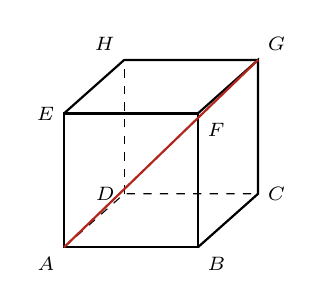
\begin{tikzpicture}[scale=0.85,font=\scriptsize]
\coordinate (A) at (0,0); \coordinate (B) at (2,0); \coordinate (C) at (2.9,0.8); \coordinate (D) at (0.9,0.8);
\coordinate (E) at (0,2); \coordinate (F) at (2,2); \coordinate (G) at (2.9,2.8); \coordinate (H) at (0.9,2.8);
\draw[thick] (A)--(B)--(F)--(E)--cycle; \draw[thick] (B)--(C)--(G)--(F); \draw[thick] (E)--(H)--(G);
\draw[dashed] (A)--(D)--(C); \draw[dashed] (D)--(H);
\draw[cThm,thick] (A)--(G);
\foreach \p/\pos in {A/below left,B/below right,C/right,D/left,E/left,F/below right,G/above right,H/above left} \node[\pos] at (\p){$\p$};
\end{tikzpicture}\end{LTR}\par}{50 د}{نرسم المكعب بالمنظور.}
\Row{}{%
\Lab{cEx}{مثال}\ في المكعب: $(AB)\parallel(HG)$ ؛ $(AB)$ و $(BF)$ متقاطعان في $B$ ؛ $(AE)$ و $(BC)$ ليسا من نفس المستوي.\par\Lab{cThm!80!black}{حذار}\ مستقيمان لا يتقاطعان ليسا بالضرورة متوازيين في الفضاء.}{}{}
\Row{التقويم}{%
\Lab{cEx}{تطبيق}\par في المكعب: حدد وضع: \Num{1} $(EF)$ و $(DC)$ ؛ \Num{2} $(AG)$ و $(EC)$ ؛ \Num{3} $(FG)$ و $(AD)$.\par\textbf{الحل:} \Num{1} متوازيان ؛ \Num{2} متقاطعان (قطرا المستطيل $AEGC$) ؛ \Num{3} متوازيان.\par\textbf{واجب منزلي:} تمارين من الكتاب المدرسي.\par\smallskip\textbf{ملاحظات حول سير الحصة:} \dotfill}{25 د}{تقويم فردي.}
\end{Sayr}
\newpage
\ModhHead{46}{1 ج م ع ت}{هندسة}{الهندسة في الفضاء}{02 سا}{الأوضاع النسبية لمستقيم ومستوٍ ولمستويين}%
{\begin{itemize}\item الأوضاع النسبية لمستقيمين.\end{itemize}}%
{\begin{itemize}\item تعيين الوضع النسبي لمستقيم ومستوٍ.\item تعيين الوضع النسبي لمستويين.\end{itemize}}%
{المنهاج ، الكتاب المدرسي ، مراجع ، مجسمات ، أدوات الهندسة.}
\begin{Sayr}
\Row{مرحلة الانطلاق}{%
\textbf{التهيئة النفسية:} قلم وورقة: بكم طريقة يمكن وضع القلم بالنسبة إلى الورقة؟}{10 د}{نشاط يدوي.}
\Row{التشخيص والاكتشاف}{%
\Lab{cEx}{مناقشة النشاطين 06 و 07 صفحة 183}\par\ck\ المستقيم $(AB)$ محتوى في المستوي $(BCGF)$ ؟ لا ، يقطعه في $B$.\par
\ck\ $(EH)$ يوازي المستوي $(ABCD)$ لأنه يوازي $(AD)$ المحتوى فيه.\par
\ck\ في الموشور: مستويان متوازيان (القاعدتان) ومستويان متقاطعان في مستقيم.\par
}{35 د}{مكعب أو موشور حقيقي.}
\Row{بناء المعارف}{%
\Lab{cThm}{مستقيم ومستوٍ}\ المستقيم إما محتوى في المستوي ، أو يوازيه تماماً ، أو يقطعه في نقطة وحيدة.\par\Lab{cThm}{مستويان}\ إما متوازيان (تماماً أو منطبقان) ، وإما متقاطعان وفق مستقيم.\par}{50 د}{نلخص الأوضاع في جدول.}
\Row{}{%
\Lab{cEx}{مثال}\ في المكعب: $(ABCD)\parallel(EFGH)$ ؛ $(ABFE)\cap(BCGF)=(BF)$ ؛ $(AE)$ يقطع $(ABCD)$ في $A$.\par\Lab{cMeth}{طريقة}\ لإثبات أن مستقيماً يوازي مستوياً يكفي أن يوازي مستقيماً من هذا المستوي.\par}{}{}
\Row{}{%
\Lab{cThm!80!black}{حذار}\ مستقيم يوازي مستوياً لا يوازي بالضرورة كل مستقيماته.}{}{}
\Row{التقويم}{%
\Lab{cEx}{تطبيق}\par في المكعب: \Num{1} وضع $(FG)$ و $(ADHE)$ ؛ \Num{2} تقاطع $(ACGE)$ و $(BDHF)$.\par\textbf{الحل:} \Num{1} $(FG)\parallel(EH)$ إذن $(FG)$ يوازي المستوي ؛ \Num{2} المستقيم الذي يشمل مركزي الوجهين $ABCD$ و $EFGH$.\par\textbf{واجب منزلي:} تمارين من الكتاب المدرسي.\par\smallskip\textbf{ملاحظات حول سير الحصة:} \dotfill}{25 د}{تقويم فردي.}
\end{Sayr}
\newpage
\ModhHead{47}{1 ج م ع ت}{هندسة}{الهندسة في الفضاء}{02 سا}{التوازي والتعامد في الفضاء}%
{\begin{itemize}\item الأوضاع النسبية.\item مبرهنة فيثاغورس.\end{itemize}}%
{\begin{itemize}\item إثبات التوازي والتعامد في الفضاء.\item حساب أطوال في مجسم.\end{itemize}}%
{المنهاج ، الكتاب المدرسي ، مراجع ، مجسمات ، أدوات الهندسة.}
\begin{Sayr}
\Row{مرحلة الانطلاق}{%
\textbf{التهيئة النفسية:} كيف يتأكد البنّاء أن العمود عمودي على الأرض؟}{10 د}{سؤال من الواقع.}
\Row{التشخيص والاكتشاف}{%
\Lab{cEx}{وضعية مقترحة}\par في المكعب $ABCDEFGH$ الذي طول حرفه $a$: \Num{1} ما وضع $(AE)$ بالنسبة إلى $(AB)$ و $(AD)$ ؟ \Num{2} احسب $AC$ ثم $AG$.\par\ck\ $(AE)$ يعامد $(AB)$ و $(AD)$ المتقاطعين في المستوي $(ABCD)$ ، فهو عمودي على هذا المستوي.\par
\ck\ $AC=a\sqrt2$ ؛ و $(CG)\perp(ABCD)$ إذن المثلث $ACG$ قائم في $C$: $AG=\sqrt{2a^2+a^2}=a\sqrt3$.\par
}{35 د}{عمل على مكعب.}
\Row{بناء المعارف}{%
\Lab{cThm}{التعامد}\ يكون مستقيم عمودياً على مستوٍ إذا عامد مستقيمين متقاطعين منه ، وعندئذ يعامد كل مستقيمات هذا المستوي.\par\Lab{cThm}{التوازي}\par\ck\ مستقيمان موازيان لمستقيم ثالث متوازيان.\par
\ck\ يتوازى مستويان إذا وازى مستقيمان متقاطعان من أحدهما المستوي الآخر.\par
}{50 د}{نرسم المثلث القائم في المكعب.}
\Row{}{%
\Lab{cEx}{مثال}\ $(CG)\perp(ABCD)$ ، إذن $(CG)\perp(AC)$.\par\smallskip\begin{LTR}\centering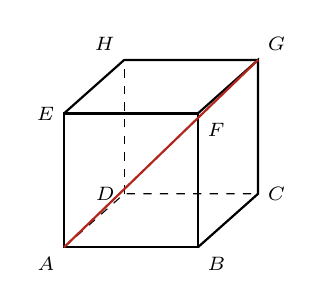
\begin{tikzpicture}[scale=0.85,font=\scriptsize]
\coordinate (A) at (0,0); \coordinate (B) at (2,0); \coordinate (C) at (2.9,0.8); \coordinate (D) at (0.9,0.8);
\coordinate (E) at (0,2); \coordinate (F) at (2,2); \coordinate (G) at (2.9,2.8); \coordinate (H) at (0.9,2.8);
\draw[thick] (A)--(B)--(F)--(E)--cycle; \draw[thick] (B)--(C)--(G)--(F); \draw[thick] (E)--(H)--(G);
\draw[dashed] (A)--(D)--(C); \draw[dashed] (D)--(H);
\draw[cThm,thick] (A)--(G);
\foreach \p/\pos in {A/below left,B/below right,C/right,D/left,E/left,F/below right,G/above right,H/above left} \node[\pos] at (\p){$\p$};
\end{tikzpicture}\end{LTR}\par\Lab{cThm!80!black}{حذار}\ لا يكفي أن يعامد المستقيم مستقيماً واحداً من المستوي.}{}{}
\Row{التقويم}{%
\Lab{cEx}{تطبيق}\par مكعب طول حرفه $10$ cm: احسب $AC$ و $AG$ ، ثم حجم الهرم $GABCD$.\par\textbf{الحل:} $AC=10\sqrt2$ ؛ $AG=10\sqrt3$ ؛ $V=\dfrac13\times100\times10=\dfrac{1000}3$ cm³.\par\textbf{واجب منزلي:} تمارين حوصلة المحور من الكتاب المدرسي.\par\smallskip\textbf{ملاحظات حول سير الحصة:} \dotfill}{25 د}{نهاية المحور: فرض أو تمارين حوصلة.}
\end{Sayr}
\end{document}
